% Numbers inserted from the campaign artifacts at freeze; macros in main.tex hold
% the reported values. Quantities written mean/sd are over the ten campaign seeds.

\begin{figure}[t]
\centering
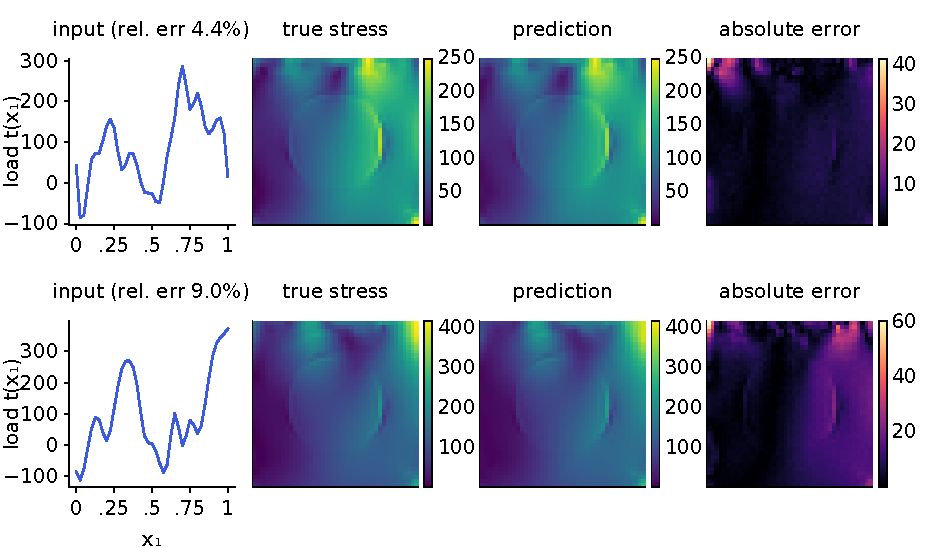
\includegraphics[width=\linewidth]{figs/fields.pdf}
\caption{Example predictions of the full pipeline. Top: a median-error test
case; bottom: a case at the 98th error percentile. Columns: input load, true
von Mises stress, prediction, and pointwise absolute error (note the smaller
scale). Errors concentrate in the high-traction corner, as also reported by
\citet{mora2025operator}.}
\label{fig:fields}
\end{figure}

\subsection{What is replicated, and at how many seeds}
\label{sec:seeds}

Every structural-mechanics number in this section is reported over ten seeds
unless it is marked otherwise. A seed here is not a reinitialization of one
network: it redraws the $1000$-sample validation split from the training pool
and reinitializes every trainable member, so the seed spread contains both the
model-selection noise and the optimization noise. The test block of $20000$
samples is fixed by the benchmark's convention and never moves, at any seed.

Five members are available at all ten seeds: the kernel ridge on loads, the
residual MLP trained on the reported metric, the same architecture trained on
normalized mean squared error, the kernel-conditioned refiner, and a Fourier
neural operator. The stack and the residual correction are run at all ten
seeds from those five, and so are the second-moment measurement and the
conformal calibration.

Two runs are incomplete, and their stopping rules are stated here once. The
FNO was stopped at every seed by the campaign's 36-hour per-task wall clock
and is finalized from the best-validation checkpoint its trainer wrote before
the stop, which falls between epochs 10 and 70 of a scheduled 200, so its
cosine schedule never annealed; nothing is retrained, and
Supplement~\ref{app:impl} records how far each run got. The one full-schedule
run of this architecture we have scored $4.705\%$ against the $\errFNOG\%$
the checkpoints average, so the truncation costs the member accuracy; the
tables report the truncated member because it is what the campaign produced.
A sixth member, a UNet, was scheduled after the FNO and completed at two of
the ten seeds before the wall clock, so the six-member configuration that
included it is not reported; as a preliminary observation only, at those two
seeds the corrected six-member pipeline scored $4.539\%$ and $4.537\%$.

The five-member set is not a configuration searched for after seeing results:
it is the pre-specified six-member configuration minus the member the campaign
could not supply. Whether five members are preferred to four is decided on
validation, per seed, by the same rule that governs every other stage choice
here, and it prefers five at ten seeds out of ten
(Section~\ref{sec:members-seeds}). The four-member pipeline is reported
alongside throughout, because the FNO's admission is a measurement and the
reader should see what it was measured against.

The low-data pipeline and the OCO-2 combination have the seed coverage stated
where they appear, which is ten in both.

\subsection{Main comparison}
\label{sec:main-results}

Table~\ref{tab:main} reports the high-data protocol. The published numbers
are quoted from \citet{dehoop2022cost} (as tabulated by
\citealt{batlle2024kernel}) and from \citet{batlle2024kernel}; our rows are
computed under the split of Section~\ref{sec:benchmark}, which gives our
methods strictly no more training information than the baselines had. The
kernel ridge row reproduces the published kernel result almost exactly
(\errKRRload\% against 5.18\%, and it is the most reproducible row in the
table: its seed standard deviation is \errKRRloadSd{} points, three thousandths
of a point, because the only randomness it carries is the validation draw).
We take that agreement as evidence that the protocols are aligned, so the gap
opened by the rest of the pipeline is not an artifact of evaluation choices.

The replicated pipeline reaches $\errPipe\pm\errPipeSd\%$, the uncertainty
being the spread over seeds. That is below every published method except
PARA-Net, and it is not separable from PARA-Net: the difference is $0.022$
points against an unpaired standard error of $\seUnpaired$
(Section~\ref{sec:uncertainty-budget}), so about one. We claim a tie there and
nothing more. Against PCA-Net (4.67\%) the separation is $0.098$
points, five standard errors, and the margins over the FNO (4.76\%), DeepONet
(5.20\%) and the optimal-recovery kernel (5.18\%) are larger still.

One correction to an earlier version of this work belongs here. That version
reported this configuration at $4.55\%$ from a single run and presented the
number as matching PARA-Net. Rebuilt across ten seeds, first without the FNO
and then with it, the pipeline gives $\errPipeFour\pm\errPipeFourSd\%$ and
$\errPipe\pm\errPipeSd\%$: the four-member figure sits three standard errors
above PARA-Net and the five-member figure is level with it, so the earlier
claim survives only at the configuration that carries the spectral member,
and only as a tie. Section~\ref{sec:diversity} presents evidence, consistent
with a floor in the benchmark data rather than a coincidence of tuning, for
why the published cluster sits where it does, and says what would settle it.

\begin{table}[t]
\centering
\caption{Structural mechanics, high-data protocol (20000 training samples,
20000 test). Mean relative $L^2$ test error. Rows above the rule are
published results on the same data, quoted without uncertainties because none
were reported. Rows below are ours: mean $\pm$ standard deviation over ten
seeds. The four-member row is the same pipeline with the FNO removed, kept
because the FNO's admission is a measurement rather than a design choice
(Section~\ref{sec:members-seeds}). TTA denotes reflection averaging at test
time.}
\label{tab:main}
\begin{tabular}{lcc}
\toprule
Method & Error (\%) & Parameters \\
\midrule
DeepONet \citep{dehoop2022cost} & 5.20 & -- \\
FNO \citep{dehoop2022cost} & 4.76 & -- \\
PCA-Net \citep{dehoop2022cost} & 4.67 & -- \\
PARA-Net \citep{dehoop2022cost} & 4.55 & -- \\
Optimal-recovery kernel \citep{batlle2024kernel} & 5.18 & -- \\
\midrule
Kernel ridge on loads (ours) & $\errKRRload\pm\errKRRloadSd$ & -- \\
Residual MLP + reflection TTA & $\errMLP\pm\errMLPSd$ & 4.9M \\
\ \ + affine stack over five members & $\errStack\pm\errStackSd$ & 22.9M \\
\ \ + residual kernel correction & $\errPipe\pm\errPipeSd$ & 22.9M \\
\ \ \ \ the same pipeline without the FNO & $\errPipeFour\pm\errPipeFourSd$ & 16.5M \\
\bottomrule
\end{tabular}
\end{table}

\begin{table}[t]
\centering
\caption{Low-data protocol (1250 training samples, 20000 test). Published
rows from \citet{mora2025operator}. Our pipeline sees only the 1250 labels
(250 of them used as the validation split). The pipeline row is mean $\pm$
standard deviation over ten seeds. Which stage the validation split selects
varies with the seed --- the input-space kernel correction at six seeds, its
two-stage form at three, the feature-space one at the remaining seed --- so
the row is the error of the selected pipeline, not of a fixed final stage.
The kernel-ridge row is a single run at the multiscale setting.}
\label{tab:lowdata}
\begin{tabular}{lc}
\toprule
Method & Error (\%) \\
\midrule
DeepONet & 8.70 \\
GP, optimal recovery \citep{batlle2024kernel} & 6.95 \\
Zero-mean GP \citep{mora2025operator} & 6.74 \\
FNO & 6.62 \\
FNO-mean GP \citep{mora2025operator} & 6.49 \\
\midrule
Kernel ridge on loads (ours, multiscale, one seed) & \errKRRloadLow \\
Full pipeline (ours, ten seeds) & $\errBestLow\pm\errBestLowSd$ \\
\bottomrule
\end{tabular}
\end{table}

\subsection{Members and the stack, across seeds}
\label{sec:members-seeds}

Table~\ref{tab:members} gives the five replicated members and the stages built
on them. Four features of it are worth naming.

The ordering of the members is stable at the top and not below it, and the
seeds are what separate the two cases. Scored on the reflection-averaged
validation predictions that the stack consumes, the normalized-MSE network is
the most accurate single member at all ten seeds --- not nine, ten. Second
place is not stable: the refiner takes it at six seeds and the FNO at four,
and on test the two are separated by $0.024$ points against the FNO's own seed
spread of $0.031$. So the first rank survives ten independent redraws of the
validation split and ten reinitializations and is not a coincidence of tuning;
the second is a coin toss that a single-seed table would have reported as a
fact. That contrast is the argument for the seeds, in one measurement.

The FNO is the interesting member, and not because it is accurate. At
$\errFNOG\pm\errFNOGSd\%$ it is third on average, behind both residual-MLP
variants, though it passes the refiner at three seeds of the ten;
its seed spread is three to five times theirs --- a consequence of
checkpoints early-stopped anywhere between epoch 10 and 70
(Supplement~\ref{app:impl}). Yet removing it costs the finished pipeline
$\fnoGain\pm\fnoGainSd$ points, and validation prefers keeping it at ten seeds
out of ten. Accuracy is not what a member contributes to a stack; the
second-moment analysis of Section~\ref{sec:diversity} says what is, and the
simplex weights there give the FNO the largest single share despite its being
third on the metric.

The stages are more reproducible than the members they are built from, and
the way the seed spread moves along the chain is itself informative: equal
weighting, which fits nothing, takes the members' spread down to $0.005$
points on test, and each subsequent fitted stage gives a little of that
back --- fitted global weights $0.006$, the affine stack \errStackSd, the
correction \errPipeSd. The end of the chain is both the most accurate
stage and the least reproducible one; fitting is not free, and a stack
tuned harder is not automatically a stack that reproduces better
(Supplement~\ref{supp:experiments}, Figure~\ref{fig:seedspread}).


Every stage gain is small and every one is resolved. Pairing within each seed on
the test set, equal weighting beats the best single member by $0.064\pm0.007$
points, fitted weights beat equal weighting by $0.021\pm0.003$, the affine stack
beats fitted global weights by $0.032\pm0.005$, and the kernel correction beats
the stack by $\corrGain\pm\corrGainSd$. All four improve at ten seeds out of
ten, as does the end-to-end figure of $\errEndToEnd\pm\errEndToEndSd$ points off
the best member the pipeline contains. Each is a few hundredths of a point,
which is precisely the resolution a single seed cannot deliver.

\begin{table}[t]
\centering
\caption{Members and stages under the high-data protocol, mean $\pm$ standard
deviation over ten seeds. Member errors are reflection-averaged where the
member has a reflection; the kernel ridge and the refiner train with the
symmetrization already applied. ``Fitted'' weights are solved on the validation
split and read out once on test; equal weights involve no fitting and are
reported on both splits.}
\label{tab:members}
\begin{tabular}{llc}
\toprule
Member or stage & Family / loss & Test error (\%) \\
\midrule
Kernel ridge on loads & Mat\'ern-$5/2$ & $\errKRRload\pm\errKRRloadSd$ \\
Residual MLP & MLP, metric loss & $\errMLP\pm\errMLPSd$ \\
Residual MLP & MLP, normalized MSE & $\errMSE\pm\errMSESd$ \\
Kernel-conditioned refiner & MLP on $(u,\mathrm{KRR}(u))$ & $\errRef\pm\errRefSd$ \\
Fourier neural operator & spectral, metric loss & $\errFNOG\pm\errFNOGSd$ \\
\midrule
Equal-weight ensemble & no fitting & $\errEnsEq\pm\errEnsEqSd$ \\
Fitted-weight ensemble & solved on validation & $\errEnsFit\pm\errEnsFitSd$ \\
Affine stack (per-pixel) & selected on a held-out half & $\errStack\pm\errStackSd$ \\
\ \ + residual kernel correction & -- & $\errPipe\pm\errPipeSd$ \\
\bottomrule
\end{tabular}
\end{table}


Three selection rules were exercised rather than assumed, and all three are
decided without touching the test block. Per-pixel affine weights are fitted on
half the validation split and accepted only if they beat global convex weights
on the other half: accepted at all ten seeds with five members, where with four
they were declined at one. The correction is accepted on validation at all ten.
And the member set itself is chosen the same way --- validation prefers five
members to four at ten seeds out of ten, which is what admits the FNO. The
test-set consequence of that last decision, $\fnoGain\pm\fnoGainSd$ points, is
read out afterwards and plays no part in making it.

\subsection{Which uncertainty is the binding one}
\label{sec:uncertainty-budget}

Seeds are not the only source of uncertainty in Table~\ref{tab:main}, and
on this benchmark they are not the largest. Every seed is scored on the
same fixed $20000$-sample test block, so the seed standard deviation
measures training and selection variability and nothing else; the test
block is itself a sample, and at a per-sample standard deviation of
$0.0169$ its contribution is $\seTest$ points, slightly larger than the
pipeline's seed spread of \errPipeSd. Treating the two as independent, the
uncertainty on our reported \errPipe\% is about $\seOwn$ points, and the
seeds contribute a little under half of it. A study that replicates seeds
and stops has measured the smaller half.

This decides what the table can support. Comparisons against a published
number are unpaired, because we do not hold those methods' per-sample
predictions, and so carry the test-block error twice: about $\seUnpaired$
points in quadrature. The separation from PCA-Net, $0.098$ points, is five
of those and real; the separation from PARA-Net, $0.022$ points, is about
one, and is therefore not a separation at all. Comparisons inside the
pipeline are paired, and pairing is worth far more here than seeds are:
the end-to-end gain of $\errEndToEnd$ points is resolved at roughly a
hundred standard errors at every seed. Supplement~\ref{supp:experiments}
works the budget through, including what it implies for the FNO's
admission; the rule it leaves is the ordinary one --- replicate seeds to
learn whether a design choice survives retraining, pair on the test set to
learn whether it helps, and never use either number to answer the other's
question.

\subsection{Architectural diversity and the shared residual}
\label{sec:diversity}

The natural reading of Table~\ref{tab:main} is that the remaining error is a
modeling problem: different architectures make different mistakes, so a more
diverse ensemble should stack to a lower number. We tested this directly, and
at every seed the measurements point the other way.

Figure~\ref{fig:corr} shows the correlation of per-sample normalized residuals
between members. Over the ten seeds every pair of members correlates between
\corrNetLo{} and \corrNetHi, and the kernel predictor --- the most alien member
by construction, an exact solve on the raw loads rather than a trained network
--- still correlates $\corrKerLo$--$\corrKerHi$ with the most accurate network.
The mean pairwise correlation is $\corrBar\pm\corrBarSd$ across seeds. The
members are not making different mistakes. They are making the same mistake
with small private variations, and how small does not depend on the seed.

The second-moment identity of Proposition~\ref{prop:secmom} makes the
consequence quantitative before any weights are fitted, and the campaign lets
us check the prediction prospectively rather than illustrate it once. At each
seed we measure the matrix $S$ of normalized residual second moments on the
validation split, solve for the optimal simplex weights, and compare the
predicted root-mean-square relative error $\sqrt{w^\top S w}$ with what those
weights realize. The prediction is $\predRMS\pm\predRMSSd\%$ and the realized
mean relative error is a factor $\dispFac\pm\dispFacSd$ of it. That factor is
the dispersion between a root-mean-square and a mean, and its stability to
three thousandths across ten independent replicates is the substantive claim:
$S$ alone, measured without ever evaluating the metric, predicts the stack.

The weights it assigns are as informative as the risk it predicts. The
optimum spreads across all five members at essentially every seed, the
kernel taking a nonzero share at ten seeds out of ten and the plain MLP at
nine; solved properly the answer is a spread, not a vertex. (An earlier
version of this work reported zero weight for those two members, from a
solver that took clipped gradient steps rather than projecting onto the
simplex.) That the FNO takes the largest single share while ranking only
third on the metric is the whole content of the diversity argument: $S$
rewards a residual that is both small and unlike the others', and the
spectral member is the only architecture here structurally unlike the
residual-MLP family. Part~(ii) of the proposition puts the
infinite-ensemble floor of an equicorrelated family at
$\bar e\sqrt{\bar\varrho}=\ensFloor\pm\ensFloorSd\%$; that is a
root-mean-square quantity and \errPipe\% is a mean, so the two are not on
the same footing and we claim no margin below the floor
(Remark~\ref{rem:metric}). What the floor measures is how little the
convex operation can buy, and the answer, at every seed, is a few
hundredths of a point. Supplement~\ref{supp:experiments} carries the
per-member weights, the pairwise admission tests, and the metric
conversion.


Where does the common mistake live? Write $r_m$ for member $m$'s residual field
on a validation case and $c=\frac1M\sum_m r_m$ for the across-member mean, the
component that no amount of uniform averaging removes. Measured over the
validation split, the shared component carries $90\%$ of the average residual
energy (Figure~\ref{fig:shared}). Three of its properties matter. Spatially,
its energy concentrates at the two corners of the loaded edge, where the
traction boundary condition meets the lateral supports; relative to the local
field scale it is three to four times larger there than the grid average, and
these are precisely the locations where the finite element solution is least
accurate and where interpolation to the $41\times41$ grid is most strained.
Spectrally, it is enriched in high radial frequencies relative to the stress
fields themselves: the fields put $97.5\%$ of their energy below radial
wavenumber 4, the shared residual only $69\%$. And its magnitude is
statistically independent of everything we can compute from the input: the
correlation of $\|c\|$ with the output norm is $0.01$, with the load norm
$0.01$, with the load's total variation $0.01$. A component that no
architecture avoids, that no input statistic predicts, that lives at the
stress concentrations, and that fixed-scale additive noise would reproduce is
consistent with noise of the data-generating process itself --- finite
element and grid-interpolation error at the singular corners --- and harder to
reconcile with approximation error of the surrogates. That is an inference,
not a demonstration: every measurement here is made on surrogates. The
experiment that would decide it is to re-solve a set of the hardest cases on
a refined mesh or with higher-order elements and compare the solver
discrepancy, case by case, with $c$; we have not run it, and the remaining
measurements in this section should be read with that in mind.

Three further measurements are consistent with the same reading, and are
reported in full in Supplement~\ref{supp:experiments}. The residual kernel
correction improves the stack by $\corrGain$ points at $n=19000$ whatever
the kernel scale, its tuner reaching for the smoothest kernel and the
largest nugget on the grid: at this sample size the shared residual is not
a function of the load in any way a Mat\'ern RKHS on $\mathbb R^{41}$ can
see. The error stops responding to data --- under identical recipes the
MLP scores $4.95\%$ at $3500$ training samples, $4.86\%$ at $8500$ and
$4.86\%$ at $19000$, so the last five-and-a-half-fold increase buys nothing
that seed noise does not already cover. And it does not respond to
reseeding either, at a scale that makes the comparison an argument: the
five published architectures of Table~\ref{tab:main} span $0.65$ points,
ten reseedings of our own pipeline $0.034$, about five percent of it. A
modeling limitation would be expected to yield to capacity, diversity,
data or reseeding; within the range we could test, this error yields to
none of them, which is the pattern a floor in the data would produce.


The spatial structure of the remaining error --- its concentration at
the corners of the loaded edge, at every seed and in every member ---
is quantified in the online supplement (Section~S3), together with
the ablation of the pipeline's stages, the error spectra, and the
cost accounting.
\subsection{Uncertainty quantification}
\label{sec:uq}
Theorem~\ref{thm:or} bounds the corrected surrogate's error by
$\|G-m\|_K\,P_\lambda(u)$, and the operator factor behaves as the theory
predicts: the fitted correction's computable squared RKHS norm is about
\normRatio$\times$ smaller when the kernel regresses ensemble residuals
than when it regresses raw stress fields, so an accurate mean genuinely
leaves a smoother remainder. The design factor $P_\lambda$ is nonetheless a
poor pointwise indicator here. It correlates \uqCorrAbs{} with the
corrected surrogate's absolute error and negatively with the benchmark's
relative error, because it tracks the output norm (\uqCorrNorm) rather
than the neural mean's mistakes, which are not a function of the
input-space geometry $P_\lambda$ sees. Ensemble disagreement, the standard
deep-ensemble signal, fails in the same direction and to the same degree
($\uqDisAbs\pm0.006$ against the absolute error, $-0.25\pm0.04$ against the
relative one), and adding the spectral member does not repair it
(\uqDisAbsFour{} on four members): disagreement measures the
member-specific error, which carries under a tenth of the residual energy,
while the shared component is invisible to any within-ensemble statistic
because the members agree precisely where they are jointly wrong
(Section~\ref{sec:diversity}).

What holds is coverage, at every seed. The exact split-conformal band is
built on $1000$ calibration cases drawn from the test block and evaluated
on the disjoint $19000$, neither used for training, checkpointing,
stacking or kernel tuning, so exchangeability holds exactly
(Section~\ref{sec:theory-conf}) and validity needs no correlation between
score and error. Observed coverage at the nominal \uqCoverNom\% level is
$\uqCover\pm\uqCoverSd\%$, and the right comparison is with the exact
finite-sample law rather than with $90\%$: the coverage of such a band is
$\mathrm{Beta}(901,100)$ distributed, whose central $95\%$ interval is
$[88.1\%,91.8\%]$, and all ten seeds fall inside it; at the $95\%$ level
the interval is $[93.6\%,96.3\%]$ and the observed coverage
$95.0\pm0.6\%$, again ten of ten. Rescaling the score by ensemble
disagreement, which the correlations say should not help, indeed does not.
Supplement~\ref{supp:experiments} carries the measurements behind each of
these statements. The lesson is narrow but real: a valid pointwise bound is
not automatically a useful pointwise indicator, two uncertainty signals of
quite different provenance can both fail on the same problem, and a
relative-error metric has to have its normalization accounted for before a
posterior standard deviation means what it appears to.
